\chapter{Quantum Circuit Optimisation}
As we saw in the previous chapters, PyZX works with quantum circuits, which are a kind of assembly language in quantum computation. They consist of primitive quantum operations (more commonly known as \textbf{gates}) applied in sequence to some quantum data (you know the drill). 

Gates take time and produce noise. So if we could do the same tasks but with \textit{fewer} gates, we win. This concept is called \textbf{quantum circuit optimisation}.

In Chapter 5, we learned how to \textbf{simplify} quantum circuits. This is, indeed, a method of optimization. And to transform these type of circuits into another with this method, we can use \textbf{spiders}.

\section{Optimisation with spiders}
Sometimes things get messy as circuits are \textit{very} rigid. Because of this, we use ZX-diagrams to simplify them! 

There's another method we could do: divide gates into smaller pieces called \textbf{spiders}. These spiders satisfy \textbf{eight} equations, which in short are called the \textbf{ZX Calculus}. In other words, \textbf{what gates are to circuits, spiders are to ZX-diagrams}. 

\begin{figure}[H]
        \centering
        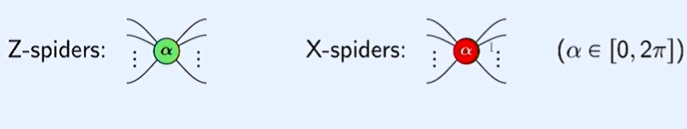
\includegraphics[width=0.5\textwidth]{Figures/spiderspic.png}
        \caption{Example of Z-spider and X-spider.}
        \label{fig:spiders.picture}
    \end{figure}
There are two types types of spiders: Z-spiders and X-spiders. They are always denoted with both colors: green and red. Now you may already understand the reason of our app's logo! 

Contrary to a quantum circuit, we can wire spiders in any way or shape you want. Therefore, \textbf{only connectivity matters}.
\begin{figure}[H]
        \centering
        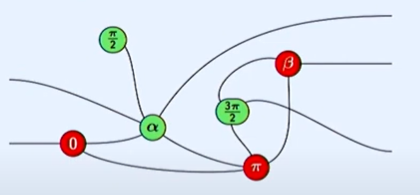
\includegraphics[width=0.5\textwidth]{Figures/example.spiders.png}
        \caption{Example of a quantum circuit using spiders.}
        \label{fig:spiders.picture}
    \end{figure}

For example, in this circuit, there are two qubits as an input and three qubits as an output. Note that we can write \textit{any} quantum gate as a ZX-diagram, so there are no excuses! Below we specify the equivalences of each gate to a spider:
\begin{figure}[H]
        \centering
        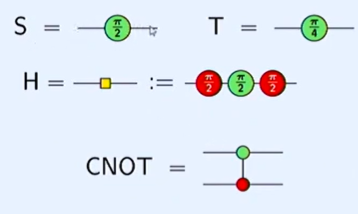
\includegraphics[width=0.5\textwidth]{Figures/equivalence.spiders.png}
        \caption{Important equivalences between gates and spiders.}
        \label{fig:eq.spiders}
    \end{figure}
So, if you remember the basics of quantum mechanics, the S gate does a quarter rotation to the qubit. $\frac{\pi}{2}$ is like a quarter rotational space ($\frac{180°}{2} = 90^\circ$, which is a quarter of 360$^\circ$). The T gate is a $\frac{1}{8}$ rotation so the spider we use is $\frac{\pi}{4}$. The Hadamard gate, on the other hand, can be decomposed in three basic rotations ($\frac{\pi}{2}$, $\frac{\pi}{2}$, $\frac{\pi}{2}$). To make this easier to read, we only use a yellow square to represent the three operations made in the qubit. Finally, the CNOT gate is solely a composition of two spiders. These are just some examples of how you can "translate" gates into spiders (actually, it was a refresher of the ZX-intro chapter). 

In the previous chapter, we could also see the rules of ZX-diagrams. Before moving on to optimisation, it is extremely important to note that if two ZX-diagrams represent the same computation, then they can be transformed into one another using the eight previous rules explained. So, instead of having dozens of \textbf{dozens} of circuit equalities, we have it much more simple now with a few simple rules! That's why ZX-Calculus is so important. The spiders "chop out" the gates in the circuit. Then, PyZX reduces it automatically using the ZX Calculus and that's it! You have successfully optimized your quantum circuit with spiders.

\begin{figure}[H]
        \centering
        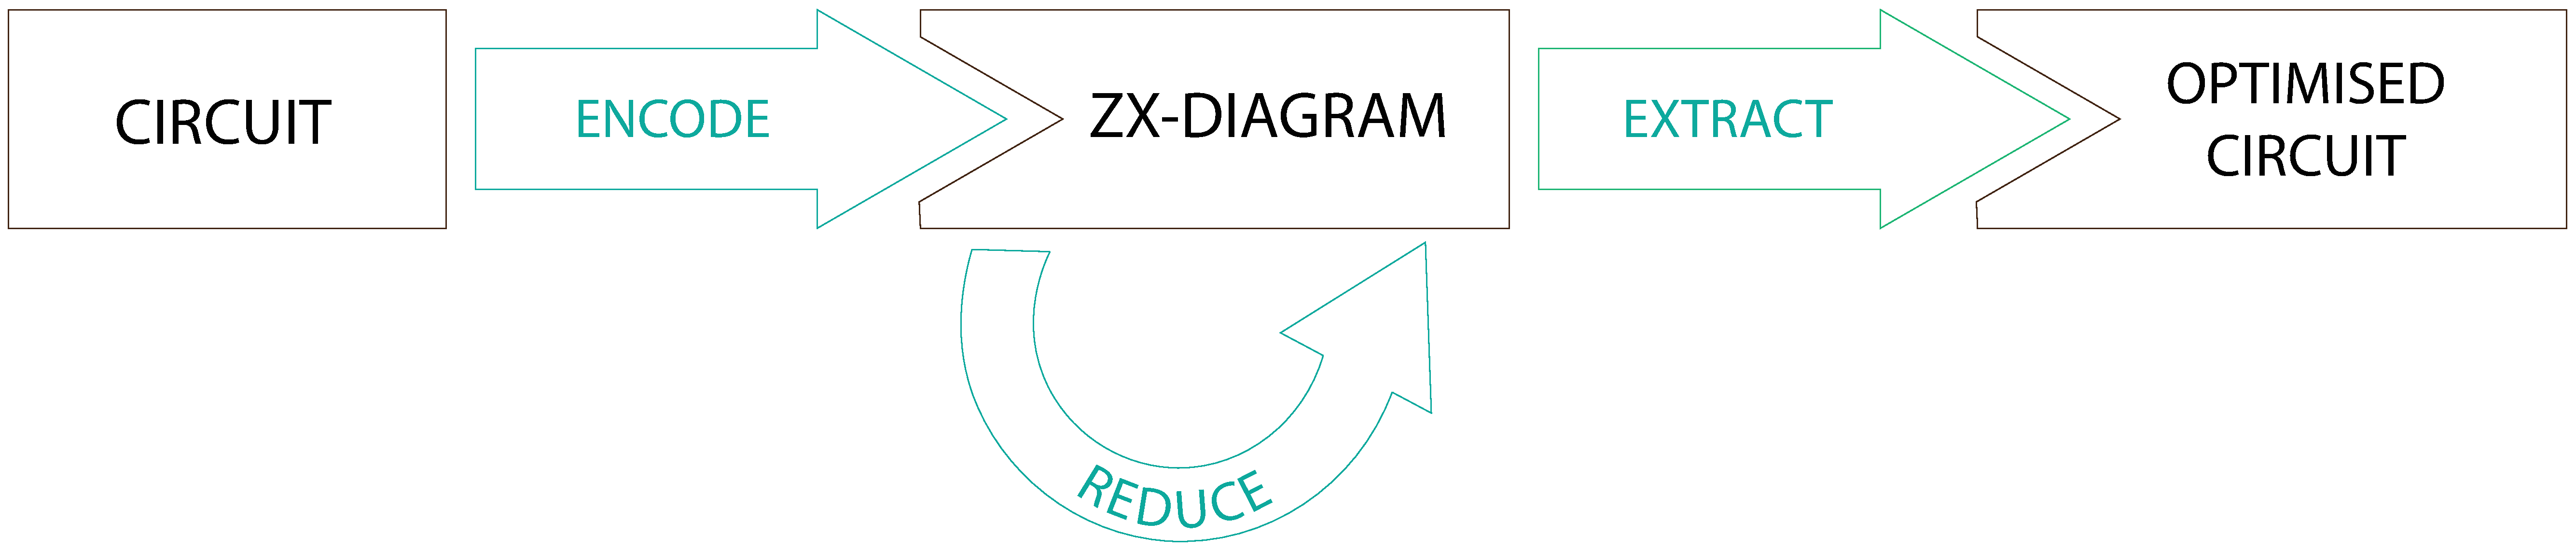
\includegraphics[width = 0.95\textwidth]{Figures/optimisation-roadmap.eps}
        \caption{ZX-diagram overall functioning}
        \label{fig:def-pyzx}
    \end{figure}

That is the main argument of ZX Calculus optimization. It is important to note that this is just an \textit{introduction} to the topic, hence we will not explain in depth the mathematics behind. However, we will be adding this material so everyone can learn it from scratch in another opportunity!

\section{Equational Rules}
\subsection{T-Rule}
The most simple way to describe it is with the concept of "only the topology matters". When spiders are in a quantum circuit, the wires may be arbitrarily organized. Still, this doesn't affect the overall computation of the program. By enumerating the inputs and outputs, any topological deformation in the middle can be simplified in a simple line. In other words, wires can be stretched or bent without consequence. If the concept doesn't "click" in your head immediately, don't worry! Here is a more visual explanation.
\begin{figure}[H]
        \centering
        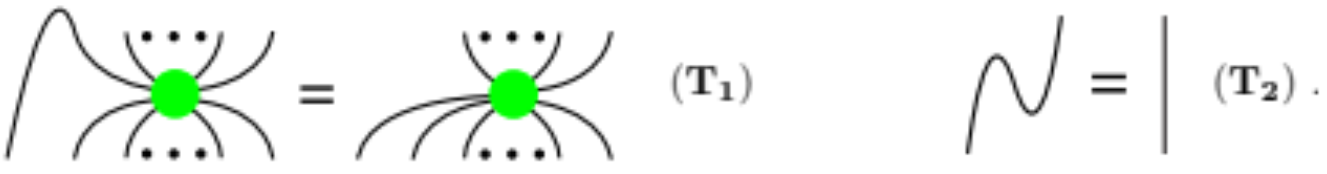
\includegraphics[width = 0.95\textwidth]{Figures/t.rule.ex.png}
        \caption{The two T-rules, T1 and T2.}
        \label{fig:t1-t2}
    \end{figure}

\begin{center}
\fcolorbox{black}{shadecolor}{%

    \parbox{\textwidth}
    {%
        \small
        {
            \textbf{Important!}
            Even though the slogan says "only the topology matters", this does NOT mean that the topology is always preserved. In fact, if you simplify a circuit, the topology will vary. The rules that we will explain may change the topology of the circuit by removing loops or even disconnecting previously connected vertices.
        }
    }%
}
\end{center}

\subsection{S-Rule}
Stands for the "spider" rule. These rules explain how dots of the \textbf{same color} interact. We have two rules:
\subsubsection{S1}
Rule S1 states that if dots of the same color are connected, they can be merged, summing the phases. Conversely, a dot can be decomposed along one or more connecting wires. Here we have a picture that illustrates the process.

\begin{figure}[H]
        \centering
        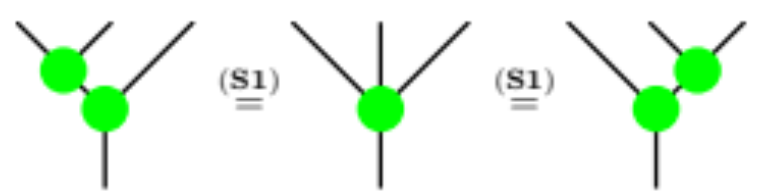
\includegraphics[width = 0.95\textwidth]{Figures/Screenshot (33).png}
        \caption{The S1 rule.}
        \label{fig:s1-rule}
    \end{figure}

\subsubsection{S2}
Rule S2 specifies when spiders are trivial. In other words, dots of degree 2 with phase $\alpha$ = 0 can be removed or, conversely, introduced.  

\subsection{B-Rule}

\subsection{K-Rule}

\subsection{C-Rule}

\subsection{D-Rule}
